\documentclass[14pt]{article} % For LaTeX2e
\usepackage{amsmath}
\usepackage{verbatim}
\usepackage{amssymb}
\usepackage{fullpage}
\usepackage{tikz} 
\usepackage{setspace}
\usepackage{amsmath}
\usepackage{amsthm}
\usepackage{amsfonts}
\usepackage{mathrsfs}
\usepackage{subfig}
\usepackage{etex}
\reserveinserts{18}
\usepackage{morefloats}
\usepackage{dsfont}
\usepackage{tikz}

\usepackage[square, numbers]{natbib}
\usepackage[colorlinks,citecolor=red]{hyperref}
%\usepackage{algorithmicx}
%\usepackage{algorithm2e}
\usepackage{algpseudocode}
\usepackage{algorithm}

\usepackage{mathtools}
\DeclarePairedDelimiter{\ceil}{\lceil}{\rceil}

\usetikzlibrary{fit,positioning}

\theoremstyle{plain}
\newtheorem{thm}{Theorem}[section]
\newtheorem{lem}[thm]{Lemma}
\newtheorem{prop}[thm]{Proposition}
\newtheorem*{cor}{Corollary}

\theoremstyle{definition}
\newtheorem{defn}{Definition}[section]
\newtheorem{ass}{Assumption}[section]
\newtheorem{conj}{Conjecture}[section]
\newtheorem{exmp}{Example}[section]
\newtheorem{exc}{Exercise}[section]


\theoremstyle{remark}
\newtheorem*{rem}{Remark}
\newtheorem*{note}{Note}


\title{MAD Style: Multivalent Authorship Detection (MAD) Topic Models for Stylometric Analysis}

\author{David Dohan, Charles Marsh, Shubhro Saha, Max Simchowitz}
\begin{document}
\maketitle
\large
\begin{abstract}
We draw a lot on \citep{Blei2007}.
\end{abstract}

\section{Introduction}

In the \textit{authorship detection} problem, one is first given a set of documents labeled (by author) on which to train, and then asked to identify authors of anonymized text snippets \citep{Stein}.

\section{Literature Review}

\section{Data}
To collect data for training and testing, we wrote scrapers for Project Gutenberg, Quora, and Nassau Weekly. We selected these three data sources for their diversity in topic, language, and length. For example, Project Gutenberg features lengthy narrative texts while Quora features shorter comments in colloquial language. With Nassau Weekly we see a mix: modern prose in a mix of narrative and editorial styles. Because of this diversity, these corpora provide ample training and testing data for our models.

We implemented our scrapers in Python. The Project Gutenberg dataset features excerpts from fiction books by five authors. The Quora dataset features about 1600 comments from roughly 100 popular Quora users. The users were selected based on online reports for ``most followed" users on the network. Because Quora is a question-answer web site, this content is mostly informative in nature. Depending on the thoroughness of a user's answer, the length can vary from a single word to several paragraphs.

The Nassau Weekly is a student-run humor/culture newspaper. Our dataset features over 550 articles from about 200 authors. The content in this dataset is largely narrative or editorial in nature, and tend to be several paragraphs in length. Interestingly, authors for the publication tend to write in vastly different tones across articles because of the unique, cultish nature of the newspaper. The challenge for our authorship models is to detect consistent features in this dataset across articles by the same author.

\section{Feature Extraction}

We incorporated six different stylometric features, each of which was composed into $n$-grams of varying sizes before being fed into the model:
\begin{enumerate}
\item Part-of-Speech (POS) tags (e.g., `Noun' for the word ``apple''). The Penn-Treebank tag set was used, and tagging itself was performed using the Maximum Entropy approach of \citet{Ratnaparkhi}.
\item Etymological tags (e.g., `Old English' for the word ``great''). Etymological information was scraped from \textit{Webster's} Dictionary \citep{Dictionary}. As etymology is inherently root-based, words absent from the dataset were first stemmatized using the method of \citet{Porter} and lemmatized using the WordNet method of \citet{Fellbaum}. If either of the results returned were present in the dictionary, their corresponding etymological tag was returned. Else, the entry with minimum Levenshtein distance was used in-place.
\item Per-syllable stress (e.g., `(0, 1, 0)' for ``continue", where a 1 indicates stress). Stresses were extracted from the CMU Pronouncing Dictionary \citep{Lenzo}. As with etymology, words absent from the dictionary were looked up by minimizing Levenshtein distance with the present keys.
\item Syllables-per-word (i.e., `3' for ``continue"), again looked-up in the CMU Pronouncing Dictionary \citep{Lenzo}.
\item Syllable counts, i.e., the total number of syllables between pieces of punctuation.
\item Word counts, i.e., the total number of words between pieces of punctuation.
\end{enumerate}

On top of these primitives, we also developed an algorithm to extract meter, inspired by \citet{Genzel}. While meter is traditionally a poetic quality (and is treated as such in \citep{Genzel}), we brought it to prose by focusing on the classical meter styles of Iambic, Spondee, etc., all of which are based on 2- or 3-syllable `feet'. We viewed meter as a function of stresses and specifically focused on the stress $(2\times3)=6$-grams, appending these $6$-grams with two additional bits: the first to indicate distance from the latest comma, and the second to indicate distance from the latest piece of punctuation. The full algorithm can be found in the Appendix.

In total, this composed seven stylometric features. For each document, we extracted these features and generated the relevant $2$-, $3$-, and $4$-grams (apart from meter, for which only $6$-grams were produced).

For illustrative purposes, Table~\ref{tab:sample_ngrams} presents several common stylistic $n$-grams and corresponding examples drawn from a Quora post by Yishan Wong, the CEO of Reddit. Notice that our feature extraction heuristics correctly identify ``Bitcoin" as a two-syllable word (despite the fact that it is not in the CMU Pronouncing Dictionary). Similarly, the etymology of ``stated" (Latin) was deduced by looking up its root, ``state"; as was the etymology of ``aims" (Old French) by looking up its root, ``aim".

\begin{table}[ht] 
\centering
\begin{tabular}{ c | c | c }
  Type & $n$-gram & Matching Text \\
  \hline
  Etymology & (AS, OE, L, OF) & ``... the key stated aims..." \\
  Syllable & (1, 1, 2, 1) & ``...fact that Bitcoin is..." \\
  Part-of-Speech & (DT, JJ, NN, IN) & ``...the libertarian culture of..." \\
  Word Counts & (7, --, 2, --) & ``It has all the features of Bitcoin--technologically speaking-- ..."
\end{tabular}
\caption{Matching stylistic $4$-grams from a Quora post.}
\label{tab:sample_ngrams}
\end{table}

\section{Methods}

To explore our data  we feed our extracted features as bags of n-grams to a novel LDA extension, the Multivalent Authorship Detection (MAD) Topic Model. The MAD topic model combines the SLDA algorithm presented in \cite{wang2009simultaneous} and \cite{Blei2007}, with the Author Topic Model in \cite{rosen2004author}, and extending both to account for multiple word types.  For each word type $t$, MAD posits its own LDA topic model. Unlike conventional LDA, in which each document shares a common Dirichlet prior, MAD gives each author her own Dirichlet prior which can be optimized with coordinate descent. This differs from the Author Topic Model, which treats each author's oeuvre as one contiguous document.

Like SLDA, MAD has a multi-class regression parameter $\eta$, from which classes are drawn from $\text{softmax}(\eta^T\bar{z})$, where $\overline{z}$ are the average topic assignments for each work. The complete generative process is specified in the Appendix, and the graphical model is show in... The key innovation in this model is that it is doubly supervised: first, each author has her own topic proportions, which enforce shared topics between her documents. And second, upon conditioning on the multi-class logistic regression $\eta$, the topic assignments $z$ which contribute to correct classification are given a higher likelihood.  Thus, one would expect that the \emph{more salient} features are selected for during inference. It is crucial to note that, during training, authorship is thereby treated as both a known label and random variable. In the test stage, however, we marginalize over authors, as described in the Appendix.

The model is fit with variational inference, discussed in \cite{wainwright2008graphical}. It is well known that exact inference for LDA requires computing a prohibitive integral \cite{Blei2003}. Instead, the posterior distribution $p(a,w,z,\theta|\alpha,\theta,\lambda,\eta)$ is approximated with a variational family: $q(\theta|\gamma)\prod_{n}q(z|\phi)$, indexed by parameters $\gamma$ and $\phi$. Here $\theta|\gamma \sim\text{Dirichlet}(\gamma)$ and $z|\phi \sim\text{Multi}(\phi)$, so that complete conditionals of $\theta$ and $z$ under $p$ are in the same family as their variational counterparts. Up to a constant independent of the variation parameters $\phi$ and $\gamma$, the KL divergence between $p$ and $q$ gives a lower bound on the posterior log likelihood. This is known as the ELBO, and (though non-convex), can be optimized with coordinate-wise gradient ascent. The parameters of the model--notably the per-author topics --can be fit using maximum likelihood methods. There are a few subtleties required to accommodate the multi-class supervision, which we defer to the appendix. The updates follow \cite{wang2009simultaneous} very closely, and in the interest of brevity, are omitted. 

After fitting the model, we extract per author distributions over topics and total corpus distribution over topics. To classify documents, we extract topic assignments by applying LDA with the model parameters fit during training, and feed the topic assignments to the logistic regression classifier. Further discussion is provided in the appendix. 

The model was implemented in C++, and based upon Chong Wang's code accompanying \cite{wang2009simultaneous}. In addition to the MAD Topic Model, our code supports L1 penalization and stochastic variational inference. Neither extensions proved particularly effective, for reasons discussed in the appendix. 
\section{Evaluation}
Note that our implementation of MAD extended Wang's implementation by 1000 C++, so preliminary testing focused on establishing the correctness of our algorithm. First, we ensured that our model likelihood increases during variational inference. Next, we simulated documents according to our generative process, and verified that we could classifiy such documents with 100\% accuracy, provided that each document had a fairly distinct distribution over topics. 

For each of the three corpora, we tested the classification accuracy sLDA against a 80/20 train/test split. We restricted our tests only to authors who had above a certain threshold of documents, which varied on the corpus. As a benchmark, we tested sLDA against Random Forest, Logistic Regression, and SVMs, appied to the back of n-grams representations of each documents. In each test, sLDA significantly outperformed an at random guess, but was outperformed by the other three benchmark methods.

\section{Conclusions}

\newpage


\begin{figure}[h!]
  \centering
  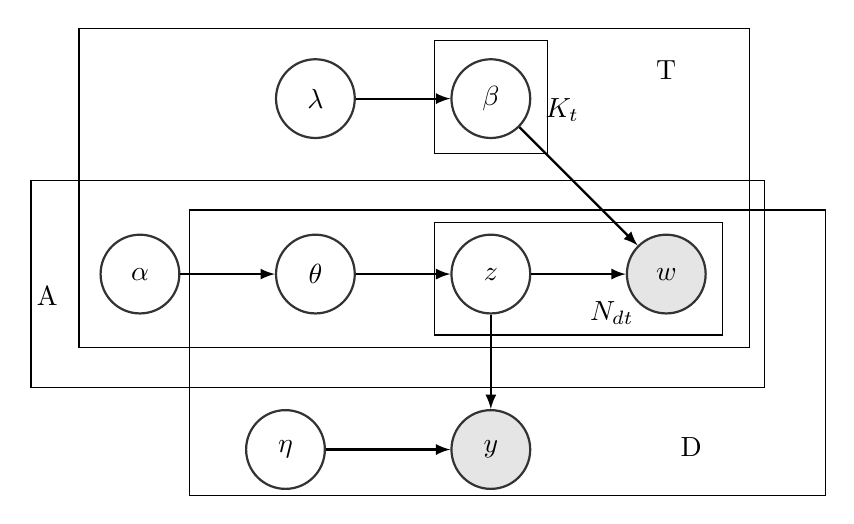
\begin{tikzpicture}
  \tikzstyle{main}=[circle, minimum size = 10mm, thick, draw =black!80, node distance = 12mm]
  \tikzstyle{connect}=[-latex, thick]
  \tikzstyle{box}=[rectangle, draw=black!100]
    \node[main, fill = white!100] (theta)  {$\theta$ };
    \node[main] (alpha) [left=of theta] { $\alpha$};
    \node[main] (z) [right=of theta] {$z$};
    \node[main, fill = black!10] (w) [right=of z] {$w$};
    \node[main] (beta) [above=of z]{$\beta$};
    \node[main] (lambda) [left=of beta]{$\lambda$};
    \node[main,  fill = black!10] (y) [below=of z,  yshift = 0mm]{$y$};
    \node[main] (eta) [left=of y, xshift = -3.8mm]{$\eta$};
    \path (alpha) edge [connect] (theta)
          (theta) edge [connect] (z)
          (z) edge [connect] (w)
          (lambda) edge [connect] (beta)
          (beta) edge [connect] (w)
          (eta) edge [connect] (y)
          (z)   edge [connect] (y);
    %\draw[->] (z.east) to  [out=-50,in=-130] (y.west) ;
    \node[rectangle, inner sep=2mm, fit= (z) (w),label=below right:$N_{dt}$, yshift = 5mm, xshift=-7mm] {};
	\node[rectangle, inner sep=2mm,draw=black!100, fit= (z) (w), yshift = -.6mm] {};
	 \node[rectangle, inner sep=2mm, fit= (beta),label= right:$K_t$, yshift = -1.4mm, xshift=-1.5mm] {};
	\node[rectangle, inner sep=2mm,draw=black!100, fit= (beta), yshift = .2mm] {};
	\node[rectangle, inner sep=8mm, fit= (theta) (z) (w) (y),label=below right:D, yshift = 16mm, xshift=-1.5mm] {};
	\node[rectangle, inner sep=13mm,minimum height = 25, draw=black!100, fit = (theta) (z) (w), yshift = -10mm, xshift=6] {};
	\node[rectangle, inner sep=8mm, fit= (alpha) (theta) (z) (w) ,label=left:A, yshift = -2.8mm, xshift=4mm] {};
	\node[rectangle, inner sep=8mm, minimum width = 60, draw=black!100, fit = (alpha) (theta) (z) (w) , yshift = -1.3mm, xshift=-2.0] {};
	\node[rectangle, inner sep=4mm, fit = (lambda) (beta) (alpha) (theta) (z) (w), label=above right:T, yshift = -8.0mm, xshift=30] {};
	\node[rectangle, inner sep=4mm, minimum width = 25, draw=black!100, fit = (lambda) (beta) (alpha) (theta) (z) (w), yshift = -.2mm, xshift=4] {};
  \end{tikzpicture}
  \caption{Graphical Model for the MAD Topic Model. Here $\alpha$ and $\lambda$ are dirichlet parameters governing distribution of topics, and per topic distributions over words. $\theta$, $z$, $\beta$ and $w$ are multinomial distributions for per-document topics, latent topic assignments, per words toics, and observed word. $y$ is a categorical glm response, with cannonical link function and parameter $\eta$. $A$ is the number of authors, $D$ the number of documents, $T$ the number of word types, $N_{dt}$ the number of words of type $t$ in document $d$, and $K_t$ the number of topics over words of type $t$.}
  \end{figure}
  \begin{algorithm}
\begin{algorithmic}[1]
\Procedure{MAD Generative Process}{}
 \State $T$ word types, with $K_t$ topics. $D$ documents, labelled into $A=$ classes, with $T$ separate word counts for each of the $T$ word types. Softmax parameter $\eta_t \in \mathbb{R}^{(A-1)\times\sum_{t=1}^TK_t}$, dirichlet priors $\{\alpha_{at}\}$ and $\{\lambda_t\}$
 	
 \For{Each Word Type $t$}
 	\State Fix vocabulary dirichlet $\lambda_t$. Draw $K_t$ topics $\beta_{tk}\sim \text{Dirichlet}(\lambda_{t})$
 \EndFor
 \For{Each Author $a$}
 	\For{Each Word Type $t$}
 	 	\State Fix author topic proportions $\alpha_{at}$
 	\EndFor
 	\For{For each document $d$ written by author $a$}
		\State Draw topic proportions $\theta_{dt}$, topics assignments $z_{dtn}$, words $w_{dtn}$ $\sim\text{LDA}(\alpha_{at},\beta_t)$.
 		\State Draw document label $\sim(\text{softmax}(\sum_{t}\overline{z}_{dt}^T\eta_t))$,where $\overline{z}_{dt}$ are average topic assignments
 	\EndFor
\EndFor
\EndProcedure
\end{algorithmic}
\end{algorithm}
\newpage
\bibliography{writeup}
\bibliographystyle{plainnat}

\newpage

\begin{appendix}
\section{Scrapers}
\section{Meter Algorithm}
\section{}


\end{appendix}

\end{document}



